%%%%%%%%%%%%%%%%%%%%%%%%%%%%%%%%%%%%%%%%%%%%%%%%%%%%%%%%%%%%%%%%
% %
% Seth Cram %
% ECE351 Section 53 %
% Lab 6 %
% Due 03/01/2022 %
% Any other necessary information needed to navigate the file %
%
%
% %
%%%%%%%%%%%%%%%%%%%%%%%%%%%%%%%%%%%%%%%%%%%%%%%%%%%%%%%%%%%%%%%%
%%%%%%%%%%%%%%%%%%%%%%%%%%%%%%%%%%%%%%%%%%%
%%% DOCUMENT PREAMBLE %%%
\documentclass[12pt]{report}
\usepackage[english]{babel}
%\usepackage{natbib}
\usepackage{url}
\usepackage[utf8x]{inputenc}
\usepackage{amsmath}
\usepackage{graphicx}
\graphicspath{{images/}}
\usepackage{parskip}
\usepackage{fancyhdr}
\usepackage{vmargin}
\usepackage{listings}
\usepackage{hyperref}
\usepackage{xcolor}
\usepackage{verbatim}
\usepackage{listings}

\definecolor{codegreen}{rgb}{0,0.6,0}
\definecolor{codegray}{rgb}{0.5,0.5,0.5}
\definecolor{codeblue}{rgb}{0,0,0.95}
\definecolor{backcolour}{rgb}{0.95,0.95,0.92}

\begin{comment} %have to use verbatim package for this

\section{Personal Notes}
            


\end{comment}

\lstdefinestyle{mystyle}{
    backgroundcolor=\color{backcolour},   
    commentstyle=\color{codegreen},
    keywordstyle=\color{codeblue},
    numberstyle=\tiny\color{codegray},
    stringstyle=\color{codegreen},
    basicstyle=\ttfamily\footnotesize,
    breakatwhitespace=false,         
    breaklines=true,                 
    captionpos=b,                    
    keepspaces=true,                 
    numbers=left,                    
    numbersep=5pt,                  
    showspaces=false,                
    showstringspaces=false,
    showtabs=false,                  
    tabsize=2
}
 
\lstset{style=mystyle}

\setmarginsrb{3 cm}{2.5 cm}{3 cm}{2.5 cm}{1 cm}{1.5 cm}{1 cm}{1.5 cm}

\title{Lab 6}		%TITLE						
% Title
\author{ Seth Cram}						
% Author
\date{02/22/2022}
% Date

\makeatletter
\let\thetitle\@title
\let\theauthor\@author
\let\thedate\@date
\makeatother

\pagestyle{fancy}
\fancyhf{}
\rhead{\theauthor}
\lhead{\thetitle}
\cfoot{\thepage}
%%%%%%%%%%%%%%%%%%%%%%%%%%%%%%%%%%%%%%%%%%%%
\begin{document}

%%%%%%%%%%%%%%%%%%%%%%%%%%%%%%%%%%%%%%%%%%%%%%%%%%%%%%%%%%%%%%%%%%%%%%%%%%%%%%%%%%%%%%%%%

\begin{titlepage}
	\centering
    \vspace*{0.5 cm}
   % \includegraphics[scale = 0.075]{bsulogo.png}\\[1.0 cm]	% University Logo
\begin{center}    \textsc{\Large   ECE 351 - 53 }\\[2.0 cm]	\end{center}% University Name
	\textsc{\Large Partial Fraction Expansion }\\[.5 cm]				% Course Code
	\rule{\linewidth}{0.2 mm} \\[0.4 cm]
	{ \huge \bfseries \thetitle}\\
	\rule{\linewidth}{0.2 mm} \\[1.5 cm]
	
	\begin{minipage}{0.4\textwidth}
		\begin{flushleft} \large
		%	\emph{Submitted To:}\\
		%	Name\\
          % Affiliation\\
           %contact info\\
			\end{flushleft}
			\end{minipage}~
			\begin{minipage}{0.4\textwidth}
            
			\begin{flushright} \large
			\emph{Submitted By :} \\
			Seth Cram  
		\end{flushright}
           
	\end{minipage}\\[2 cm]
	
\end{titlepage}

%%%%%%%%%%%%%%%%%%%%%%%%%%%%%%%%%%%%%%%%%%%%%%%%%%%%%%%%%%%%%%%%%%%%%%%%%%%%%%%%%%%%%%%%%

\tableofcontents
\pagebreak

%%%%%%%%%%%%%%%%%%%%%%%%%%%%%%%%%%%%%%%%%%%%%%%%%%%%%%%%%%%%%%%%%%%%%%%%%%%%%%%%%%%%%%%%%
\renewcommand{\thesection}{\arabic{section}}

\section{Introduction}

The goal of lab 6 is to utilize a function from the scipy module to perform partial fraction expansion using Python in the Spyder IDE.

\section{Equations}
    \begin{equation}
        u(t) = \{t<0:0, t>=0:1\}
    \end{equation}
 
    \begin{equation}
        u(s) = 1/s
    \end{equation}
 
    \begin{equation}
       H(s) = Y (s)/X(s) = (s^2 + 6s + 12)/((s + 4)(s + 6))
    \end{equation}
    
     \begin{equation}
        y(t) = (0.5 − 0.5 \cdot e^{−4t} + e^{-6t} ) \cdot u(t)
    \end{equation}
    
    \begin{equation}
        Y (s) = (s^2 + 6s + 12)/(s(s + 4)(s + 6))
    \end{equation}
    
    \begin{equation}
        H(s) = 25,250/(s^6+18s^5+218s^4+2036s^3+9085s^2+25,250s)
    \end{equation}
\section{Methodology}

%This section will describe how you went about solving the lab. Make sure you go into detail about any method you used. %Include coding samples here if necessary. This is also where you would include necessary derivations. An example of %inserting code into the report is given. Do not go overboard on inserting code into your report, only use whats %absolutely necessary to illustrate your point.

    \paragraph{} First, I completed the prelab. This required some partial fraction expansion without complex roots. The results of which can be viewed from Equation three and four. 
    \paragraph{} Moving onto the lab, I plotted the step response of H(s), equation four. Then, I actually used H(s), equation three, to plot the step response using scipy.signal.step(). 
    \paragraph{} Then, I input Y(s), equation five, from the prelab into scipy.signal.residue() to find the partial fraction expansion. Comparing this result with what I found through doing it by hand, they were the exact same. Comparison was difficult at first, but after understanding that R was roots and P was poles, it was a simple matter. 
    \paragraph{} For the complicated system presented next, I found the partial fraction expansion of the step response using the residue function. Using this result, I initially tried to use the sin-method by-hand to plot the time-domain response. When that failed, I switched over to the cos-method implemented as a user-defined Python function and found the correct result. I'm still unsure as to why the sin-method didn't work properly or where I was going wrong. 
    \paragraph{} I know this function was the correct one because I compared it to using the signal.step function on H(s) from equation 6. I made sure to plot both functions on the same graph for easy comparison.  
    
\section{Results}

%This section will go over the results of the lab. Use this area to describe %if the lab worked as expected or if the results are unexpected or different %from your hand calculations or intuition. Part of being a good engineer is %gaining intuition about these problems and being able to understand quickly %if something is wrong. Use code, plots, tables, and figures as necessary. %Make sure to cite all other works used and note them in the bibliography. A %sample entry is in this document.

    \paragraph{} I plotted from 0 to 2 seconds and expected both my function and the library computed function to be the same because I had no reason to believe they should be different. 
    
    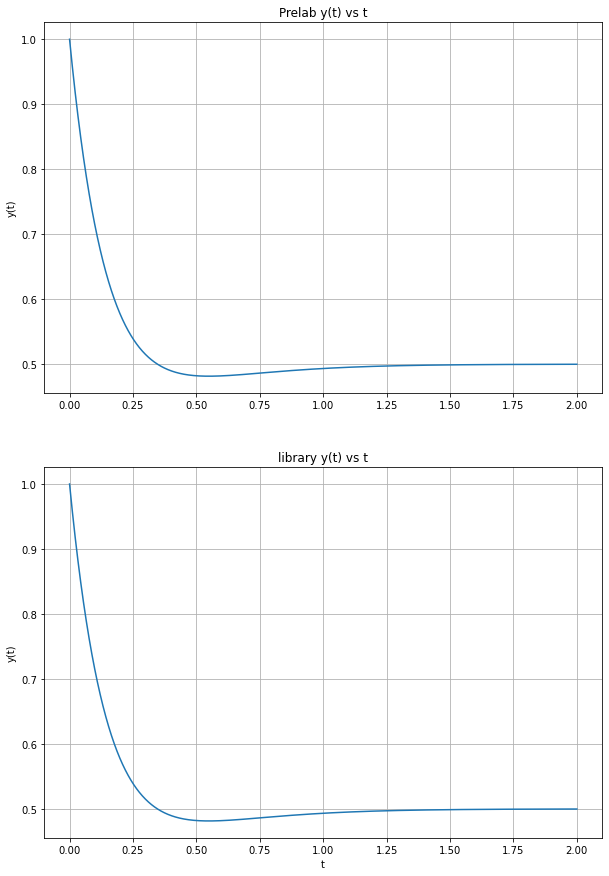
\includegraphics[scale=0.6]{prelab compare.png}
    
    \paragraph{} My expectation held true. Although Python functions have given us different output in the past, this case wasn't one of those instances. All aspects of the graphs are the exact same.  
    
    \paragraph{} My expectation for the complicated system's step response was that they'd be exactly the same. The scaling, shape and overall flow should hold true since they all did previously during this lab.
    
    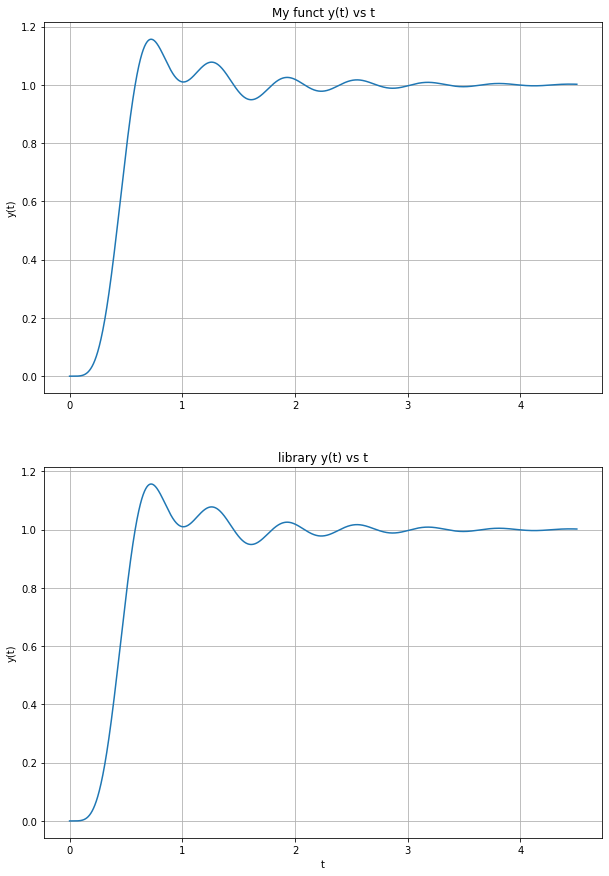
\includegraphics[scale=0.6]{complicated compare.png}
    
    \paragraph{} Impressively enough, even with complex roots, my function and the library function output the exact same curves. 


\section{Error Analysis}

%This section will discuss error analysis of the experiment. Since this lab %deals with ideal simulation there shouldn't be any sources of error, so %instead this section can be used to describe any difficulties you had during %lab and how you solved them. Alternatively, if you couldn't get the %experiment to work, which is okay, you need to use this section to explain why %you couldn't get it to work to earn full points. 

\paragraph{} A possible source of error could be rounding done when I hand calculated the complicated system using the sin-method. Another possible source of error for the sin-method could have been the usage of multiple complex roots and not using the correct equations for that scenario.  

\paragraph{} The main difficulty I encountered was trying to get the sin-method to work properly. When I decided it wasn't worth the continued effort, my next biggest difficulty was trying to understand how the cos-method worked. Up until lab, I didn't understand how the cos-method worked whatsoever. So, the learning curve was somewhat steep.  

\section{Questions} %also address any deliverables not yet put in yet
    \begin{enumerate}
        \item . For a non-complex pole-residue term, you can still use the cosine method, explain why this
works.
        \paragraph{} The cosine method still works for non-complex poles because the cosine term just becomes one since the coefficient on t becomes zero. This results in an exponential and step function term, the same as one would get using an inverse laplace table. 
        
        \item Leave any feedback on the clarity of lab tasks, expectations, and deliverables
        \paragraph{} The clarity of the prelab and deliverables was great. The expectations were a bit more ambiguous. Since the lab handout specified the usage of the cos-method and we'd only used it once in class before, it was difficult to tell if it was okay to use the sin-method or not.  
    \end{enumerate}

\section{Conclusion}

%Discuss briefly what you learned in this lab and whether or not you feel the %lab was successful. Include any recommendations for future labs as this is a %learning experience for all of us. Discuss any insights you gained from this %lab and how that will affect future work. \textit{Note: The bibliograhpy %needs to be on its own page.}

    \paragraph{} During lab 6, I went through the step response of a simple and complicated system. In summary, I learned more about how to use tuples in Python to input to a function and capture output from a function, how to use the cos-method in a useful manner, and what the gain of a system means. The lab was somewhat successful, since I still don't understand whether the sin-method is a viable option for the complicated system, and why it isn't if so. Having experience with the cos-method will be useful when dealing with complex roots from now on. It's always good to know two ways to solve a problem.  
    
    Github: \url{https://github.com/SethCram} 
    
%\newpage


\appendix

\chapter{Simple Function}
     Console output:
    \begin{lstlisting}
        partial fraction results:  [ 0.5 -0.5  1. ]
        Corresponding poles:  [ 0. -4. -6.]
        Coeffs of the direct polynomial terms:  []  
    \end{lstlisting}
 
 \chapter{Complex Function}
    Console output:
    \begin{lstlisting}
        partial fraction results:  [ 1.+0.j         -0.48557692+0.72836538j    -0.48557692-0.72836538j     -0.21461963+0.j          0.09288674-0.04765193j  0.09288674+0.04765193j]
        Corresponding poles:  [  0.+0.j  -3.+4.j  -3.-4.j -10.+0.j  -1.+10.j  -1.-10.j]
        Coeffs of the direct polynomial terms:  []        
    \end{lstlisting}

\newpage

\end{document}